\documentclass[a4paper,12pt]{article}
\usepackage[a4paper,top=1.3cm,bottom=2cm,left=1.5cm,right=1.5cm,marginparwidth=0.75cm]{geometry}
\usepackage{cmap}
\usepackage{mathtext}
\usepackage[T2A]{fontenc}
\usepackage[utf8]{inputenc}
\usepackage[english,russian]{babel}
\usepackage{siunitx}
\usepackage{enumitem}
\usepackage{placeins}

\usepackage{graphicx}

\usepackage{wrapfig}
\usepackage{tabularx}
\usepackage{multirow}

\usepackage{hyperref}
\usepackage[rgb]{xcolor}
\hypersetup{
colorlinks=true,urlcolor=blue
}
\usepackage{siunitx}
\usepackage{amsmath,amsfonts,amssymb,amsthm,mathtools}
\usepackage{icomma}
\mathtoolsset{showonlyrefs=false}
\usepackage{euscript}
\usepackage{mathrsfs}
\DeclareMathOperator{\sgn}{\mathop{sgn}}
\newcommand*{\hm}[1]{#1\nobreak\discretionary{}
{\hbox{$\mathsurround=0pt #1$}}{}}

%%% Заголовок
\newcommand\labname{Интерферометр Фабри-Перо}
\newcommand\labnumber{4.4.4}


\author{Макаров Лев Евгеньевич}
\title{Лабораторная работа №\labnumber

\labname
}

\date{\today}

\begin{document}

\begin{titlepage}
	\begin{center}
		{\large МОСКОВСКИЙ ФИЗИКО-ТЕХНИЧЕСКИЙ ИНСТИТУТ (НАЦИОНАЛЬНЫЙ ИССЛЕДОВАТЕЛЬСКИЙ УНИВЕРСИТЕТ)}
	\end{center}
	\begin{center}
		{\large Физтех-школа фотоники, электроники и молекулярной физики}
	\end{center}
	
	
	\vspace{4.5cm}
	{\huge
		\begin{center}
			{\bf Отчёт о выполнении лабораторной работы \labnumber}\\
			\labname
		\end{center}
	}
	\vspace{2cm}
	\begin{flushright}
		{\LARGE Автор:\\ Макаров Лев Евгеньевич \\
			\vspace{0.2cm}
			Б04-306}
	\end{flushright}
	\vspace{8cm}
	\begin{center}
		Долгопрудный 2025
	\end{center}
\end{titlepage}


\section{Введение}

\textbf{Цель работы:} 
\begin{enumerate}
	\item Определение характеристик интерферометра Фабри-Перо: база интерферометра, добротность, линейная дисперсия, аппаратная разрешающая способность
    \item Определение числа интерферирующих лучей, разности длин волн для линий пары колец.
\end{enumerate}

\textbf{В работе используются:} ртутная и натриевая лампы, интерферометры Фабри-Перо, катетометры, линзы, светофильтры, оптические скамьи.

\section{Теоретические сведения}

\FloatBarrier
\begin{figure}[!h]
	\begin{minipage}[h]{0.55\linewidth}
		\center{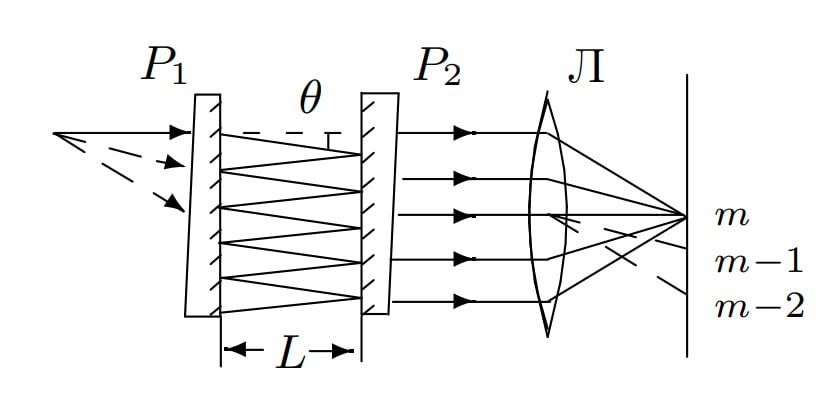
\includegraphics[width=0.95\linewidth]{ifp.png}}
	\end{minipage}
	\begin{minipage}[h]{0.5\linewidth}
		\center{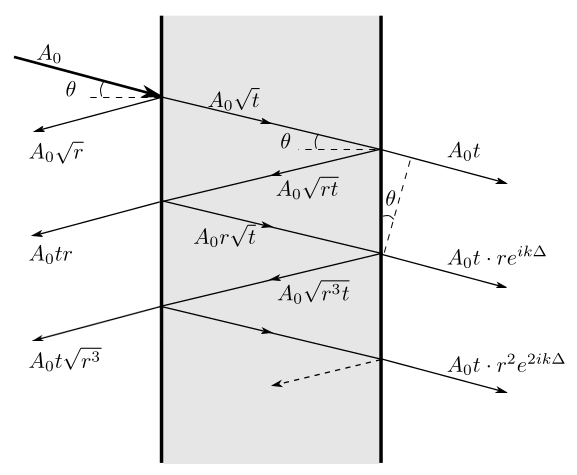
\includegraphics[width=0.95\linewidth]{fp.png}}
	\end{minipage}
  \caption[]{\label{fig:ifp} Интерферометр Фабри-Перо}
\end{figure}
\FloatBarrier

Интерферометр Фабри–Перо состоит из двух стеклянных (или кварцевых) пластин P1 и P2,
внутренние плоские поверхности которых
хорошо отполированы (с точностью до $10^{-2}\lambda$) и установлены параллельно друг
другу. На эти поверхности наносятся хорошо отражающие покрытия. Наружные поверхности
пластин обычно составляют небольшой угол с внутренними, чтобы световой блик,
отраженный от наружных поверхностей, не мешал наблюдениям. Интерферометр Фабри–Перо можно
рассматривать как плоскопараллельную воздушную пластину, на которой происходят
многократные отражения и интерференция световых лучей. Интерференционная картина,
наблюдаемая в фокальной плоскости линзы Л, состоит из концентрических колец равного
наклона. Для двух соседних лучей, распространяющихся между зеркалами интерферометра
под углом $\theta$, разность хода определяется соотношением

\begin{align*}
    \Delta = 2L\cos\theta
\end{align*}

где $L$ --- расстояние между зеркалами.
Разрешающей способностью прибора называют величину

\begin{align*}
    R = \frac{\lambda}{\delta\lambda}
\end{align*}

разрешающая способность характеризует возможность прибора различать
две близкие спектральные линии с длинами волн $\lambda$ и $\lambda+\delta\lambda$

Угловая дисперсия определяется как

\begin{align*}
    D = \frac{d\varphi}{d\lambda}
\end{align*} 

По величине угловой дисперсии можно определить угловое расстояние между двумя
близкими спектральными линиями: $\delta\varphi = D\delta\lambda$

Дисперсионная область – предельная ширина спектрального интервала $\Delta\lambda$ прибора, для которой дифракционные максимумы соседних порядков не перекрываются. Она определяет диапазон
длин волн, при которых прибор может быть использоан для анализа спектра.

В случае интерферометра Фабри-Перо интерференционные
максимумы будут наблюдаться для волн, падающих под углами $\theta_{m}$, удовлетворяющими
условию:

\begin{equation}\label{max_inter}
    2L\cos{\theta_{m}} = m\lambda,
\end{equation}

где $L$ - база интерферометра. Для малых углов выражение можно переписать как 

\begin{equation}
    \label{eq:1}
    \theta_m^2 = 2 - \frac{\lambda}{L}m
\end{equation}

Так как  $\theta(i) = \frac{d(i)}{2f}$, где $f$ --- фокусное расстояние линзы, стоящей после интерферметра, а $d(i)$ --- диаметр i-ого кольца, можно
получить зависимость угла на максимум интерференции от его номера или диаметра кольца 

\begin{equation}
    \label{eq:2}
    \frac{d^2(i)}{4f^2} = \theta^2(i) = \text{const} + \frac{i\lambda}{L}
\end{equation}

Выражение можно преобразовать для получения угловой дисперсии:

\begin{equation}
    D_{\text{угл}} \approx -\frac{1}{\lambda \theta_{m}},
\end{equation}

где $\theta_{m} = \frac{d}{2f}$ в данной работе ($f$ -- фокусное расстояние используемой в работе линзы).

Также для малых углов условие возникновения  интерференционного кольца можно записать в виде:

\begin{equation}
    \frac{\lambda}{L} = \frac{1}{4f^2}\frac{\Delta(d^2_i)}{\Delta(i)},
\end{equation}

Отсюда следует используемая в работе формула для линейной дисперсии, которая используется в работе:

\begin{equation}
    D = \frac{2f^{2}}{\lambda d}
\end{equation}

Аппаратная разрешающая способность для порядка спектра $m \approx \frac{2L}{\lambda}$ может быть найдена как:

\begin{equation}
    R = \frac{\lambda}{\delta \lambda} = \frac{\pi \sqrt{r}}{1 - r}m = Nm,
\end{equation}

где $N = \dfrac{\pi \sqrt{r}}{1 - r}$ -- число интерферирующих лучей.

Дисперсионная область интерферометра Фабри-Перо может быть найдена по следующей формуле:

\begin{equation}
    \Delta \lambda = \frac{\lambda^{2}}{2L}.
\end{equation}

\section{Экспериментальная установка}

В работе используются ртутная и натриевая лампы; интерферометры Фабри-Перо,
катетометры, линзы, светофильтры, оптические скамьи.

\FloatBarrier
\begin{figure}[htbp]
    \centerline{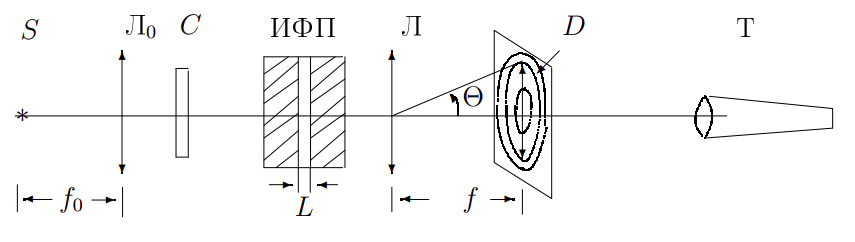
\includegraphics[width=0.7\textwidth]{ust.png}}
    \caption[]{\label{fig:scheme} Схема установки}
\end{figure}
\FloatBarrier

На схеме $S$ --- лампа, $ Л_0 $ --- линза, $ C $ --- светофильтр, ИФП --- интерферометр
Фабри-Перо, $T$ --- зрительная труба. Диаметры колец измеряются с помощью микроскопа
катетометра.

\section{Результаты измерений и обработка данных}

\subsection*{I. Юстировка системы}

\begin{enumerate}
    \item Включим лампу.
    \item Убедимся, что на интерферометр попадает свет.
    \item В остальном установка является настроенной
    \item Ознакомимся с техническим описанием приборов
\end{enumerate}

\subsection*{II. Измерения}

\begin{enumerate}[resume]
    \item Замерим диаметры колец и запишем в таблицы \ref{table:1}-\ref{table:4}
\end{enumerate}

\FloatBarrier
\begin{table}[!ht]
    \centering
    \caption{Измерение диаметров колец зеленой пары Ртутной лампы}
    \begin{tabular}{|l|l|l|l|}
        \hline
        $N_{down}$ & $x_{down}$, мм & $N_{up}$ & $x_{up}$, мм   \\ \hline
        1       & 169.290 & -1    & 184.361 \\ \hline
        2       & 165.989 & -2    & 187.624 \\ \hline
        3       & 163.536 & -3    & 190.000 \\ \hline
        4       & 161.517 & -4    & 192.028 \\ \hline
        5       & 159.769 & -5    & 193.752 \\ \hline
        6       & 158.237 & -6    & 195.295 \\ \hline
        7       & 156.788 & -7    & 196.703 \\ \hline
        8       & 155.512 & -8    & 197.964 \\ \hline
        9       & 154.333 &       &         \\ \hline
        10      & 153.210 &       &         \\ \hline
    \end{tabular}
    \label{table:1}
\end{table}
\FloatBarrier

\FloatBarrier
\begin{table}[!ht]
    \centering
    \caption{Измерение диаметров колец Натриевой лампы}
    \begin{tabular}{|l|l|l|l|}
        \hline
        $N_{down}$ & $x_{down}$, мм & $N_{up}$ & $x_{up}$, мм   \\ \hline
        4       & 141.915 & -4    & 161.000 \\ \hline
        5       & 140.272 & -5    & 162.449 \\ \hline
        6       & 139.420 & -6    & 163.327 \\ \hline
        7       & 138.209 & -7    & 164.652 \\ \hline
        8       & 137.493 & -8    & 165.281 \\ \hline
        9       & 136.354 & -9    & 166.421 \\ \hline
        10      & 135.800 & -10   & 166.973 \\ \hline
        11      & 134.727 & -11   & 168.074 \\ \hline
        12      & 134.265 & -12   & 168.632 \\ \hline
        13      & 133.301 &       &         \\ \hline
        14      & 132.771 &       &         \\ \hline
        15      & 131.860 &       &         \\ \hline
        16      & 131.450 &       &         \\ \hline
    \end{tabular}
    \label{table:2}
\end{table}
\FloatBarrier

\FloatBarrier
\begin{table}[!ht]
    \centering
    \caption{Измерение диаметров колец оранжевой пары Ртутной лампы}
    \begin{tabular}{|l|l|l|l|}
        \hline
        $N_{down}$ & $x_{down}$, мм & $N_{up}$ & $x_{up}$, мм   \\ \hline
        8       & 160.925 & 8     & 192.618 \\ \hline
        9       & 159.655 & 9     & 193.790 \\ \hline
        10      & 159.100 & 10    & 194.355 \\ \hline
        11      & 158.000 & 11    & 195.421 \\ \hline
        12      & 157.600 & 12    & 195.873 \\ \hline
        13      & 156.610 & 13    & 196.839 \\ \hline
        14      & 156.140 & 14    & 197.276 \\ \hline
        15      & 155.279 &       &         \\ \hline
        16      & 154.866 &       &         \\ \hline
        17      & 153.935 &       &         \\ \hline
        18      & 153.657 &       &         \\ \hline
    \end{tabular}
    \label{table:3}
\end{table}
\FloatBarrier

\FloatBarrier
\begin{table}[!ht]
    \centering
    \caption{Измерение диаметров колец желтой пары Ртутной лампы}
    \begin{tabular}{|l|l|l|l|}
        \hline
        $N_{down}$ & $x_{down}$, мм & $N_{up}$ & $x_{up}$, мм   \\ \hline
        8       & 160.911 & -8    & 192.714 \\ \hline
        9       & 159.661 & -9    & 193.921 \\ \hline
        10      & 159.073 & -10   & 194.483 \\ \hline
        11      & 158.080 & -11   & 195.552 \\ \hline
        12      & 157.507 & -12   & 196.015 \\ \hline
        13      & 156.528 & -13   & 196.960 \\ \hline
        14      & 156.126 & -14   & 197.439 \\ \hline
        15      & 155.194 &       &         \\ \hline
        16      & 154.801 &       &         \\ \hline
        17      & 153.973 &       &         \\ \hline
        18      & 153.562 &       &         \\ \hline
    \end{tabular}
    \label{table:4}
\end{table}
\FloatBarrier

\clearpage

\begin{enumerate}[resume]
    \item Замерим $\delta r$ для желтой, зеленой пары ртути и для натрия. Запишем результаты в таблицу \ref{table:5}.
\end{enumerate}

\FloatBarrier
\begin{table}[!ht]
    \centering
    \caption{Измерение $\delta r$ для разный пар}
    \begin{tabular}{|l|l|l|l|}
        \hline
        ~              & желтый  & зелены  & натрий  \\ \hline
        $x_{up}$, мм   & 183.822 & 184.392 & 156.166 \\ \hline
        $x_{down}$, мм & 184.099 & 184.714 & 156.666 \\ \hline
        $\delta r$, мм & 0.277   & 0.322   & 0.500   \\ \hline
    \end{tabular}
    \label{table:5}
\end{table}
\FloatBarrier

\begin{enumerate}[resume]
    \item Оценим максимальный порядок интерференции и дисперсионную область
\end{enumerate}

\begin{enumerate}[resume]
    \item данный пункт не выполнялся
\end{enumerate}

\subsection*{III. Обработка результатов}

\begin{enumerate}
    \item Построим график зависимости $d_i^2 = F(i)$ для зеленой пары ртути. Изобразим его на рисунке \ref{graph:1}
\end{enumerate}

\FloatBarrier
\begin{figure}[!h]
    \centering
    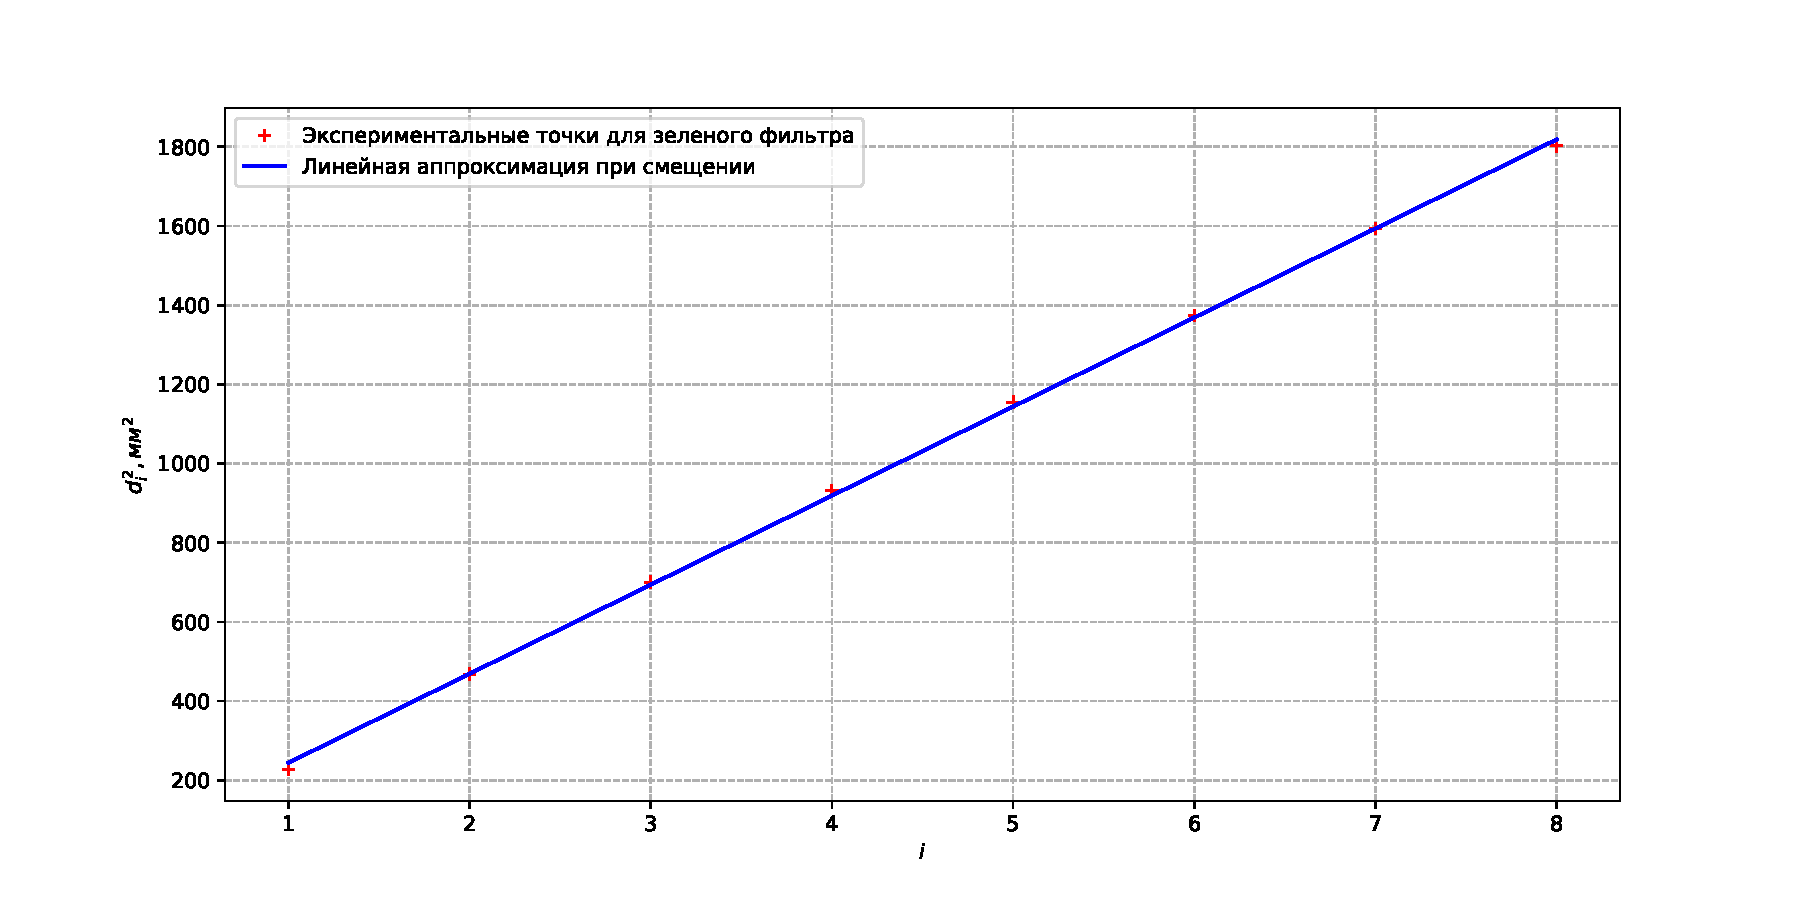
\includegraphics[scale=0.65]{graph_green.pdf}
    \caption{График зависимости $d_i^2 = F(i)$ для зеленой пары}
    \label{graph:1}
\end{figure}
\FloatBarrier

Рассчитаем базу интерферометра:

\begin{equation*}
    L = \frac{4\lambda f^2}{k} \approx (0.118 \pm 0.005) \ \text{мм}
\end{equation*}

\clearpage

\begin{enumerate}[resume]
    \item Построим график зависимости $\overline{d} = F(1/\Delta d)$ и изобразим его на рис. \ref{graph:2}
\end{enumerate}

\FloatBarrier
\begin{figure}[!h]
    \centering
    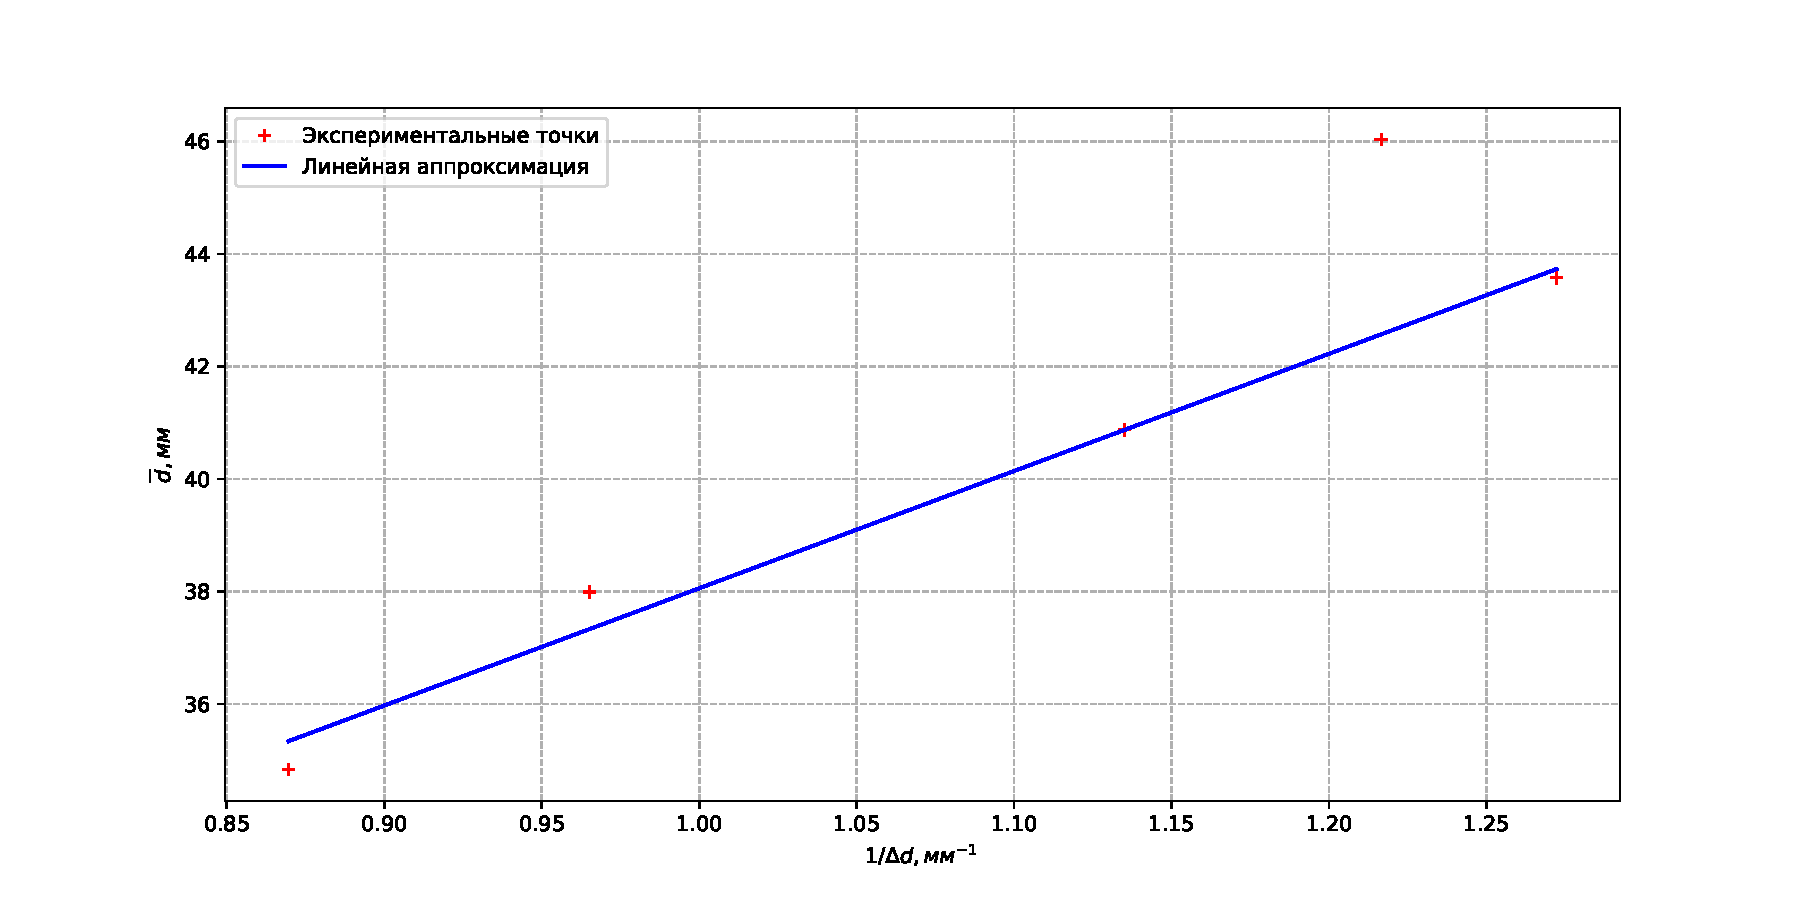
\includegraphics[scale=0.65]{graph_yellow.pdf}
    \caption{График зависимости $\overline{d} = F(1/\Delta d)$ для желтой пары линий ртути}
    \label{graph:2}
\end{figure}
\FloatBarrier

По углу наклона рассчитаем разность длин волн $\Delta \lambda$ для желтой пары

\begin{equation*}
    \Delta \lambda = \frac{\lambda k}{4 f^2} \approx 2.5 \ \text{\si{\angstrom}}
\end{equation*}

\begin{enumerate}[resume]
    \item Построим аналогичные графики и аналогичные рассчеты для натриевой лампы.
\end{enumerate}

\begin{equation*}
    L = \frac{4\lambda f^2}{k} \approx (0.279 \pm 0.005) \ \text{мм}
\end{equation*}

\begin{equation*}
    \Delta \lambda = \frac{\lambda k}{4 f^2} \approx 3.2 \ \text{\si{\angstrom}}
\end{equation*}

\FloatBarrier
\begin{figure}[!h]
    \centering
    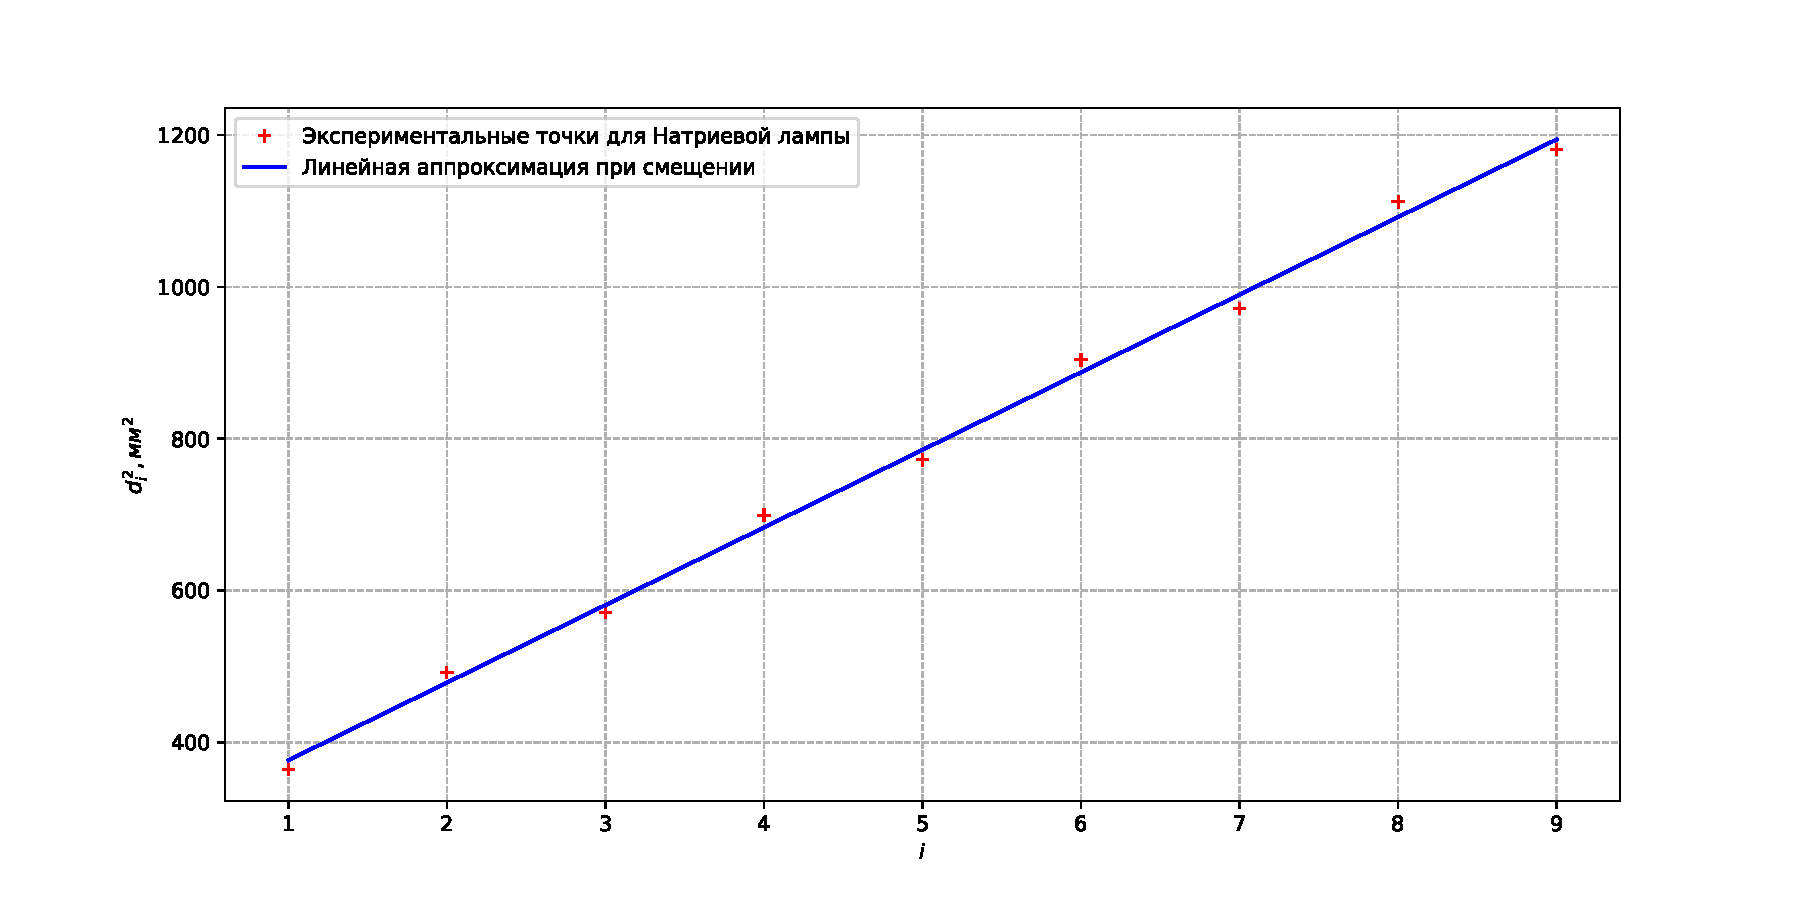
\includegraphics[scale=0.65]{graph_na_1.pdf}
    \caption{График зависимости $d_i^2 = F(i)$ для линий натрия}
    \label{graph:3}
\end{figure}
\FloatBarrier

\FloatBarrier
\begin{figure}[!h]
    \centering
    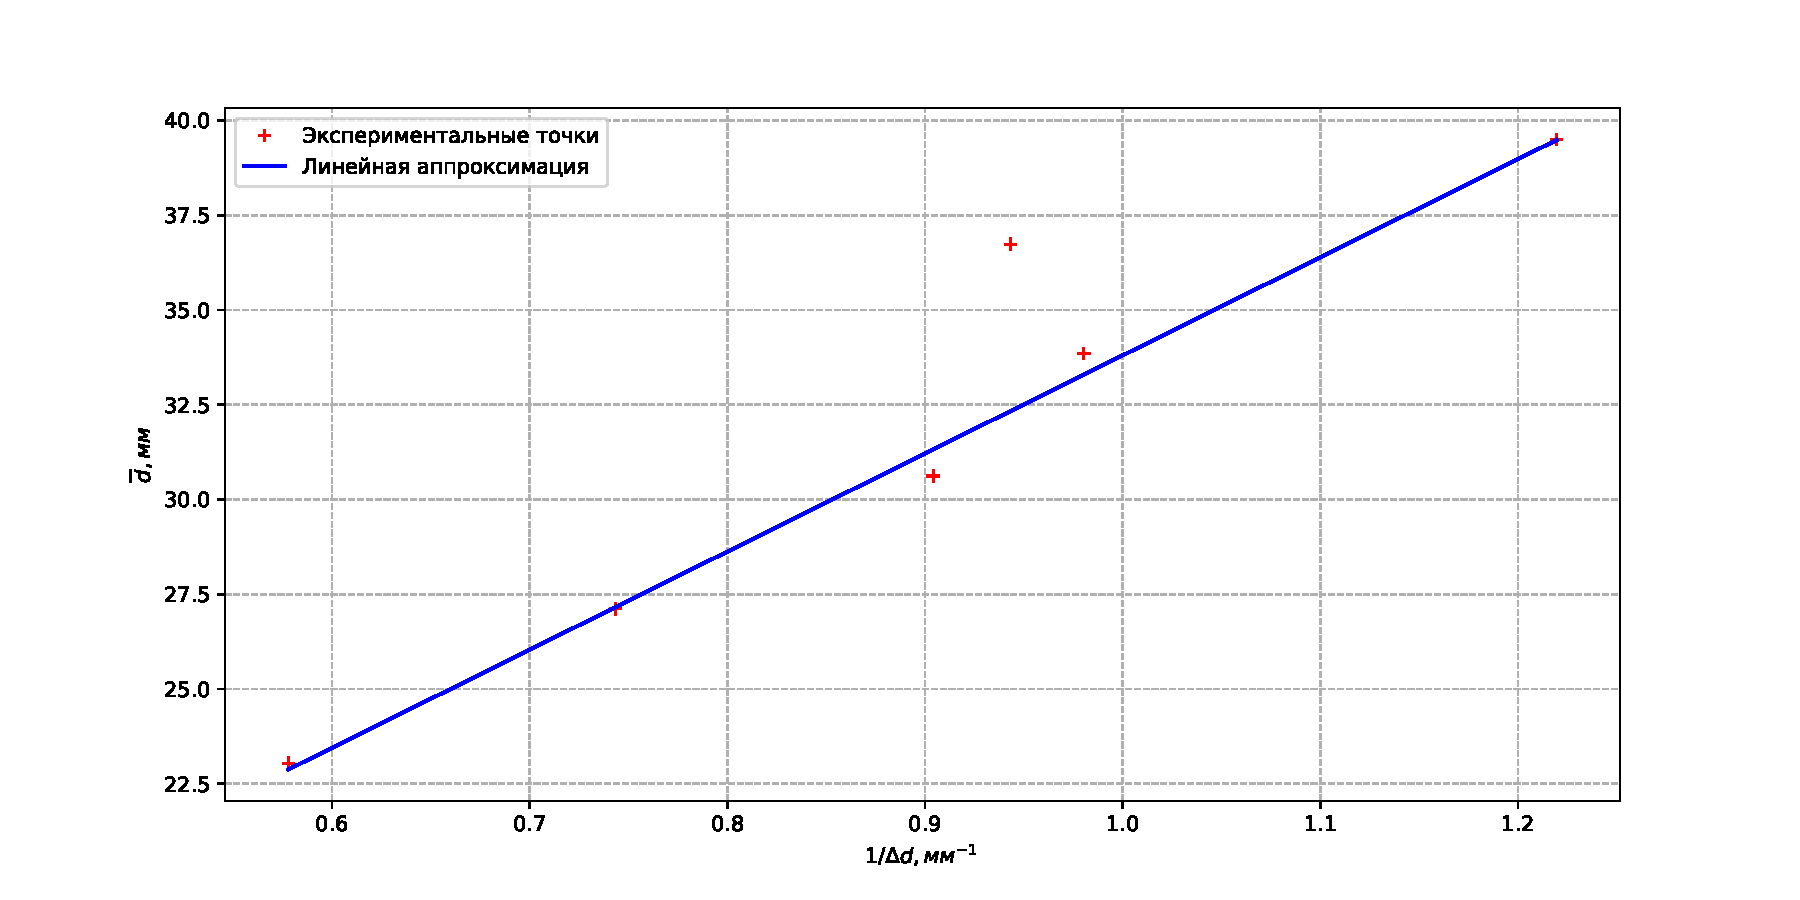
\includegraphics[scale=0.65]{graph_na_2.pdf}
    \caption{График зависимости $\overline{d} = F(1/\Delta d)$ для линий натрия}
    \label{graph:4}
\end{figure}
\FloatBarrier

\clearpage

\begin{enumerate}[resume]
    \item Оценим экспериментальное значение линейной дисперсии интерферометра. Результаты запишем в таблицу \ref{table:6} для желтой пары и таблицу \ref{table:7} для натрия.
\end{enumerate}

\FloatBarrier
\begin{table}[!ht]
    \centering
    \caption{Измерение $D$ для желтой пары}
    \begin{tabular}{|l|l|l|l|l|l|}
        \hline
        $N$ & 1     & 2     & 3     & 4     & 5     \\ \hline
        $D_{exp}$, мм/\si{\angstrom}     & 0.231 & 0.208 & 0.177 & 0.158 & 0.165 \\ \hline
        $D_{theor}$, мм/\si{\angstrom}   & 0.120 & 0.110 & 0.102 & 0.096 & 0.091 \\ \hline
    \end{tabular}
    \label{table:6}
\end{table}
\FloatBarrier


\FloatBarrier
\begin{table}[!ht]
    \centering
    \caption{Измерение $D$ для натрия}
    \begin{tabular}{|l|l|l|l|l|l|l|}
        \hline
        $N$ & 1     & 2     & 3     & 4     & 5  & 6   \\ \hline
        $D_{exp}$, мм/\si{\angstrom}     & 0.274 & 0.213 & 0.175 & 0.162 & 0.168 & 0.130 \\ \hline
        $D_{theor}$, мм/\si{\angstrom}   & 0.178 & 0.151 & 0.134 & 0.121 & 0.112 & 0.104 \\ \hline
    \end{tabular}
    \label{table:7}
\end{table}
\FloatBarrier


\begin{enumerate}[resume]
    \item Оценим аппаратную разрешающую способность 
\end{enumerate}

\begin{equation*}
    R_{Na} = \frac{4 f^2}{D \delta r} \approx 3500
\end{equation*}

\begin{equation*}
    R_{Рп} = \frac{4 f^2}{D \delta r} \approx 2000
\end{equation*}




\end{document}
